\section{Thảo luận và phân tích lỗi}

\subsection{Hiện tượng Overfitting / Underfitting}

Dựa trên kết quả Learning Curves và so sánh Train/Test performance, nhóm nhận xét trạng thái từng mô hình:

\begin{table}[H]
\centering
\caption{Phân tích Overfitting / Underfitting và biện pháp khắc phục}
\label{tab:overfitting}
\resizebox{\textwidth}{!}{
\begin{tabular}{|l|l|l|}
\hline
\textbf{Mô hình} & \textbf{Trạng thái} & \textbf{Biện pháp khắc phục} \\
\hline
Logistic Regression & Ổn định (low bias, low variance) & Regularization L2 (C=10) \\
Linear SVC & Ổn định & Regularization L2, class\_weight=balanced \\
Multinomial NB & Underfitting nhẹ & Smoothing alpha=0.1 \\
Random Forest & \textbf{Overfitting} (train$\approx$1.0, val$\approx$0.94) & class\_weight=balanced, SMOTE \\
SGD Classifier & Ổn định & L2 penalty, 20 epochs \\
PhoBERT & \textbf{Overfitting nhẹ} (val loss tăng epoch 2--3) & Weight decay=0.01, 3 epochs \\
\hline
\end{tabular}
}
\end{table}

\textbf{Random Forest} thể hiện overfitting rõ nhất (Hình~\ref{fig:lc_rf}): train F1$\approx$1.0 nhưng val F1$\approx$0.94. Nguyên nhân là RF có thể ghi nhớ toàn bộ tập train khi \texttt{max\_depth=None}. Biện pháp khắc phục đã thử gồm giới hạn \texttt{max\_depth} (thử 10, 30, 50) và \texttt{class\_weight='balanced'}, tuy nhiên hiệu quả cải thiện hạn chế.

\textbf{PhoBERT} có dấu hiệu overfitting nhẹ: Training Loss liên tục giảm nhưng Validation Loss tăng từ epoch 2. Nhóm sử dụng \texttt{load\_best\_model\_at\_end=True} và \texttt{weight\_decay=0.01} để giảm thiểu.

Hình~\ref{fig:overfitting} minh họa phân tích overfitting thông qua so sánh Train score và Val/Test score.

\begin{figure}[H]
\centering
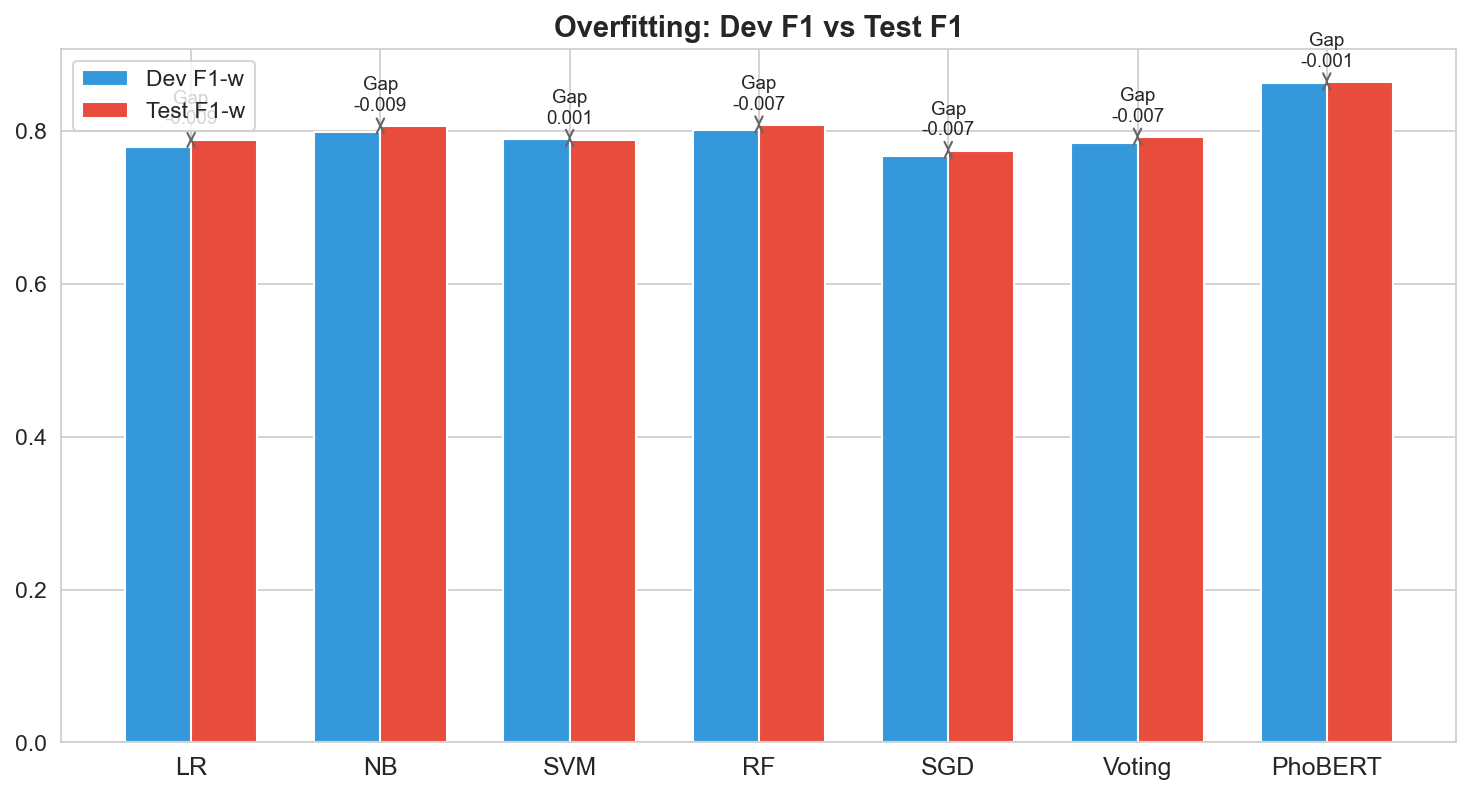
\includegraphics[width=0.7\textwidth]{figures/overfitting_analysis.png}
\caption{Phân tích Overfitting: so sánh Train CV Score và Test F1-weighted}
\label{fig:overfitting}
\end{figure}

%---------------------------------------------------
\subsection{Phân tích các trường hợp sai}

Mô hình PhoBERT-base-v2 dự đoán sai \textbf{941 / 6{,}527 mẫu} (14.4\%) trên tập Test. Bảng~\ref{tab:error_types} phân nhóm 5 loại nhầm phổ biến nhất.

\begin{table}[H]
\centering
\caption{Top 5 loại nhầm lẫn phổ biến nhất (PhoBERT trên tập Test)}
\label{tab:error_types}
\begin{tabular}{|l|l|c|l|}
\hline
\textbf{Nhãn thực} & \textbf{Nhãn dự đoán} & \textbf{Số mẫu} & \textbf{Giả thuyết nguyên nhân} \\
\hline
CLEAN & OFFENSIVE & 275 & Chứa từ nhạy cảm hoặc phóng đại nhưng ngữ cảnh trung tính \\
CLEAN & HATE & 266 & Chứa từ khóa thường gặp ở bình luận thù ghét nhưng mang ý thảo luận \\
HATE & CLEAN & 136 & Sử dụng ngôn từ thù ghét gián tiếp, châm biếm, ẩn ý tinh vi \\
OFFENSIVE & CLEAN & 120 & Ranh giới mờ nhạt giữa ngôn từ thân mật bình thường và xúc phạm nhẹ \\
OFFENSIVE & HATE & 91 & Nhầm lẫn cường độ công kích cá nhân với thù ghét nhóm đối tượng \\
\hline
\end{tabular}
\end{table}

\textbf{Nhận xét:} Do sử dụng Weighted Cross-Entropy Loss để phạt nặng hơn lỗi trên các lớp thiểu số (HATE và OFFENSIVE), mô hình có xu hướng dự đoán nhạy bén hơn cho các lớp này, dẫn đến một lượng đáng kể mẫu CLEAN bị phân loại nhầm thành OFFENSIVE (275 mẫu) và HATE (266 mẫu). Đây là sự đánh đổi (trade-off) điển hình khi giải quyết mất cân bằng dữ liệu: chấp nhận giảm Precision của lớp đa số để tối đa hóa Recall cho lớp thiểu số quan trọng.

Hình~\ref{fig:error_dist} hiển thị phân bố các loại lỗi.

\begin{figure}[H]
\centering
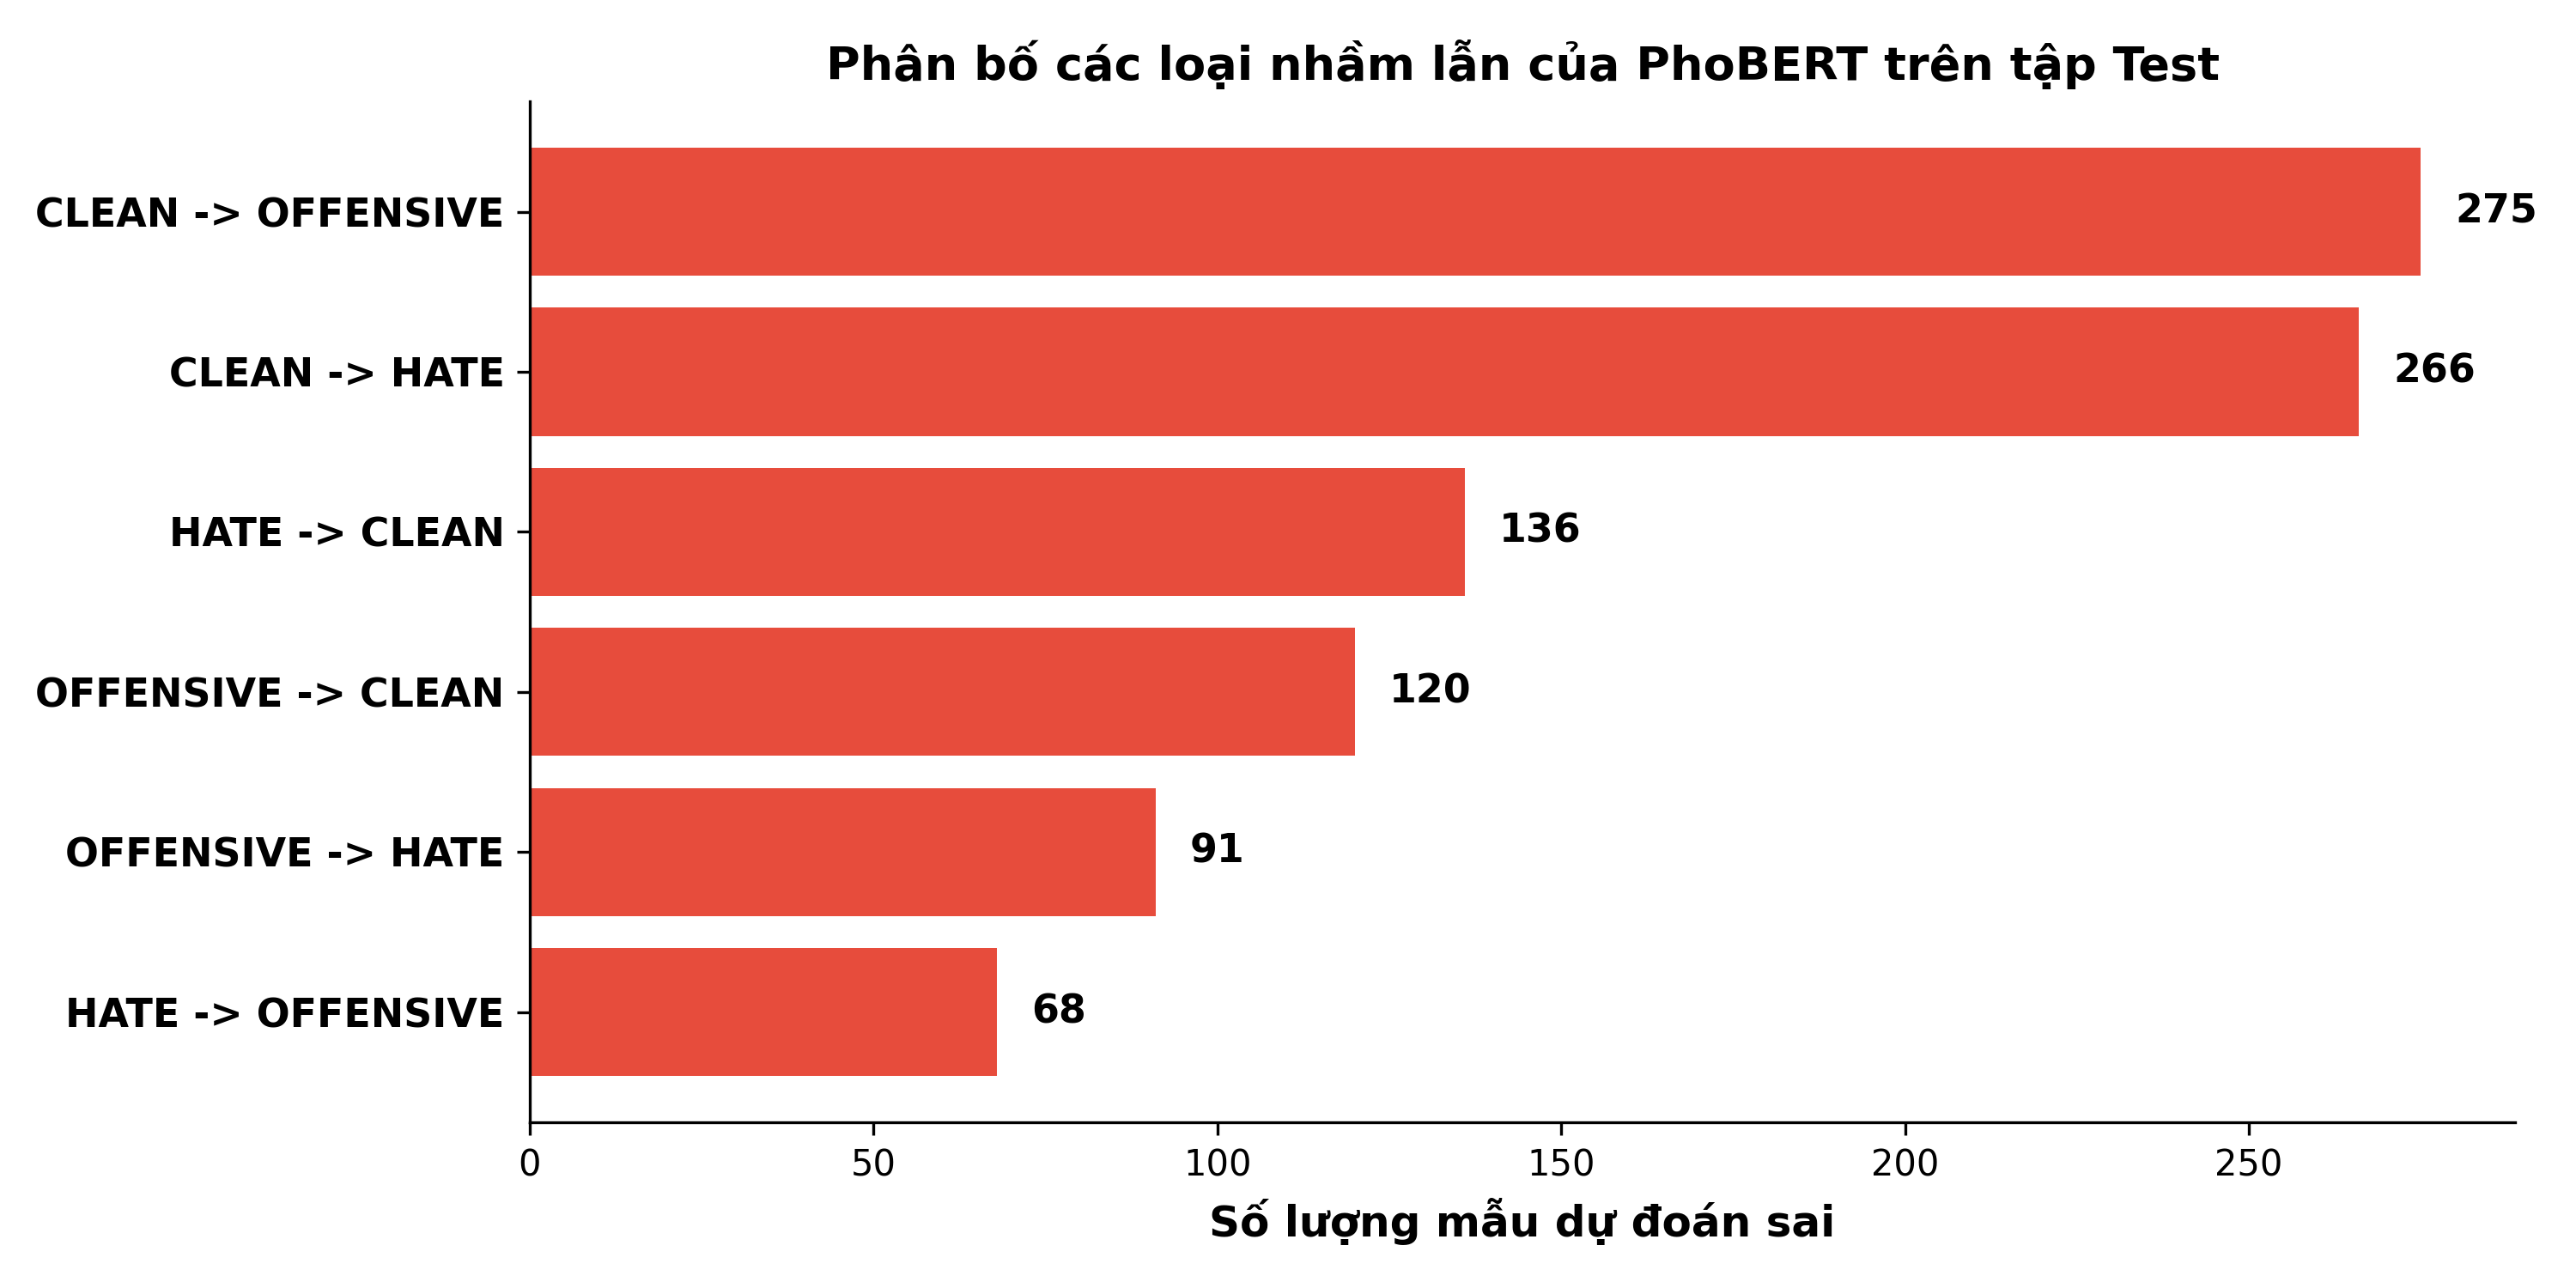
\includegraphics[width=0.65\textwidth]{figures/error_distribution.png}
\caption{Phân bố các loại nhầm lẫn của PhoBERT trên tập Test}
\label{fig:error_dist}
\end{figure}

\subsubsection{Các ví dụ cụ thể về lỗi phân loại}

Để làm rõ hơn hành vi của mô hình, Bảng~\ref{tab:error_examples} trình bày các ví dụ thực tế được trích xuất từ tập Test bị PhoBERT phân loại sai, cùng với lý do phân tích chi tiết.

\begin{table}[H]
\centering
\caption{Các ví dụ thực tế bị PhoBERT phân loại sai trên tập Test}
\label{tab:error_examples}
\resizebox{\textwidth}{!}{
\begin{tabular}{|p{6cm}|c|c|p{7cm}|}
\hline
\textbf{Văn bản bình luận} & \textbf{Thực tế} & \textbf{Dự đoán} & \textbf{Phân tích lỗi} \\
\hline
\textit{"bữa nay nhìn ngon dữ thần nha"} & CLEAN & OFFENSIVE & Từ "ngon" thường xuất hiện trong ngữ cảnh bình luận thô tục, gợi dục (OFFENSIVE). Mô hình chưa nhận diện được sắc thái khen ngợi thân mật trong câu này. \\
\hline
\textit{"thằng này ăn tàn phá hại cả một thế hệ học sinh"} & OFFENSIVE & CLEAN & Câu mang tính công kích cá nhân cao nhưng không chứa các từ chửi tục trực tiếp. Do đó, mô hình bỏ sót sắc thái xúc phạm này. \\
\hline
\textit{"tụi này chỉ biết làm khổ đất nước thôi, đuổi hết đi"} & HATE & CLEAN & Ngôn từ thù ghét gián tiếp nhắm vào một nhóm người (xenophobia/hate speech). Vì không dùng từ tục tĩu thô thiển nên mô hình không nhận ra tính thù ghét. \\
\hline
\textit{"đúng là đồ óc chó không biết suy nghĩ gì"} & OFFENSIVE & HATE & Từ công kích cá nhân nặng ("óc chó") bị mô hình phân loại nhầm thành HATE do nhầm lẫn giữa xúc phạm cá nhân nặng và thù ghét nhóm đối tượng. \\
\hline
\end{tabular}
}
\end{table}

%---------------------------------------------------
\subsection{Bảng so sánh hiệu năng giữa các mô hình}

Bảng~\ref{tab:model_compare} so sánh toàn diện hiệu năng trên cả Dev và Test, kèm F1-score theo từng lớp.

\begin{table}[H]
\centering
\caption{So sánh hiệu năng giữa các mô hình (sắp xếp theo Test F1-weighted)}
\label{tab:model_compare}
\begin{tabular}{|l|c|c|c|c|}
\hline
\textbf{Mô hình} & \textbf{Dev F1-w} & \textbf{Test F1-w} & \textbf{Best CV Score} & \textbf{Ranking} \\
\hline
\textbf{PhoBERT-base-v2} & \textbf{0.8629} & \textbf{0.8637} & - & \textbf{1} \\
Random Forest & 0.8016 & 0.8080 & 0.9418 & 2 \\
Multinomial NB & 0.7982 & 0.8068 & 0.6632 & 3 \\
Voting Ensemble & 0.7853 & 0.7919 & - & 4 \\
Logistic Regression & 0.7795 & 0.7899 & 0.8932 & 5 \\
Linear SVC & 0.7901 & 0.7889 & 0.9033 & 6 \\
SGD Classifier & 0.7676 & 0.7746 & 0.7452 & 7 \\
\hline
\end{tabular}
\end{table}

\textbf{Phân tích về Rò rỉ dữ liệu (Data Leakage):} Nhóm nhận thấy \texttt{Best CV Score} của các mô hình truyền thống (đặc biệt là Random Forest đạt 0.9418, Linear SVC đạt 0.9033, và Logistic Regression đạt 0.8932) cao hơn rất nhiều so với hiệu năng thực tế trên tập Test (chỉ quanh mức 0.78--0.80). 

Nguyên nhân chính của hiện tượng này là do \textbf{rò rỉ dữ liệu (data leakage)} trong quá trình tinh chỉnh siêu tham số bằng \texttt{GridSearchCV}. Cụ thể, SMOTE đã được áp dụng để cân bằng lớp trên toàn bộ dữ liệu huấn luyện \textbf{trước khi} thực hiện phân chia các fold cho Cross-Validation. Khi các mẫu nhân tạo được sinh ra dựa trên khoảng cách của dữ liệu gốc, việc chia fold ngẫu nhiên sau đó sẽ khiến các mẫu nhân tạo rất giống nhau xuất hiện đồng thời ở cả fold huấn luyện (Train fold) và fold kiểm thử (Validation fold). Điều này làm cho điểm số Cross-Validation bị thổi phồng giả tạo (overestimated). 

Để khắc phục triệt để hiện tượng này trong các dự án thực tế, SMOTE cần được nhúng trực tiếp vào một pipeline huấn luyện (ví dụ: sử dụng \texttt{imblearn.pipeline.Pipeline} thay vì \texttt{sklearn.pipeline.Pipeline}) để đảm bảo SMOTE chỉ được áp dụng trên tập huấn luyện của fold đó và hoàn toàn độc lập với fold kiểm thử.


Hình~\ref{fig:f1_per_class} so sánh F1-score theo từng lớp cho 6 mô hình truyền thống.

\begin{figure}[H]
\centering
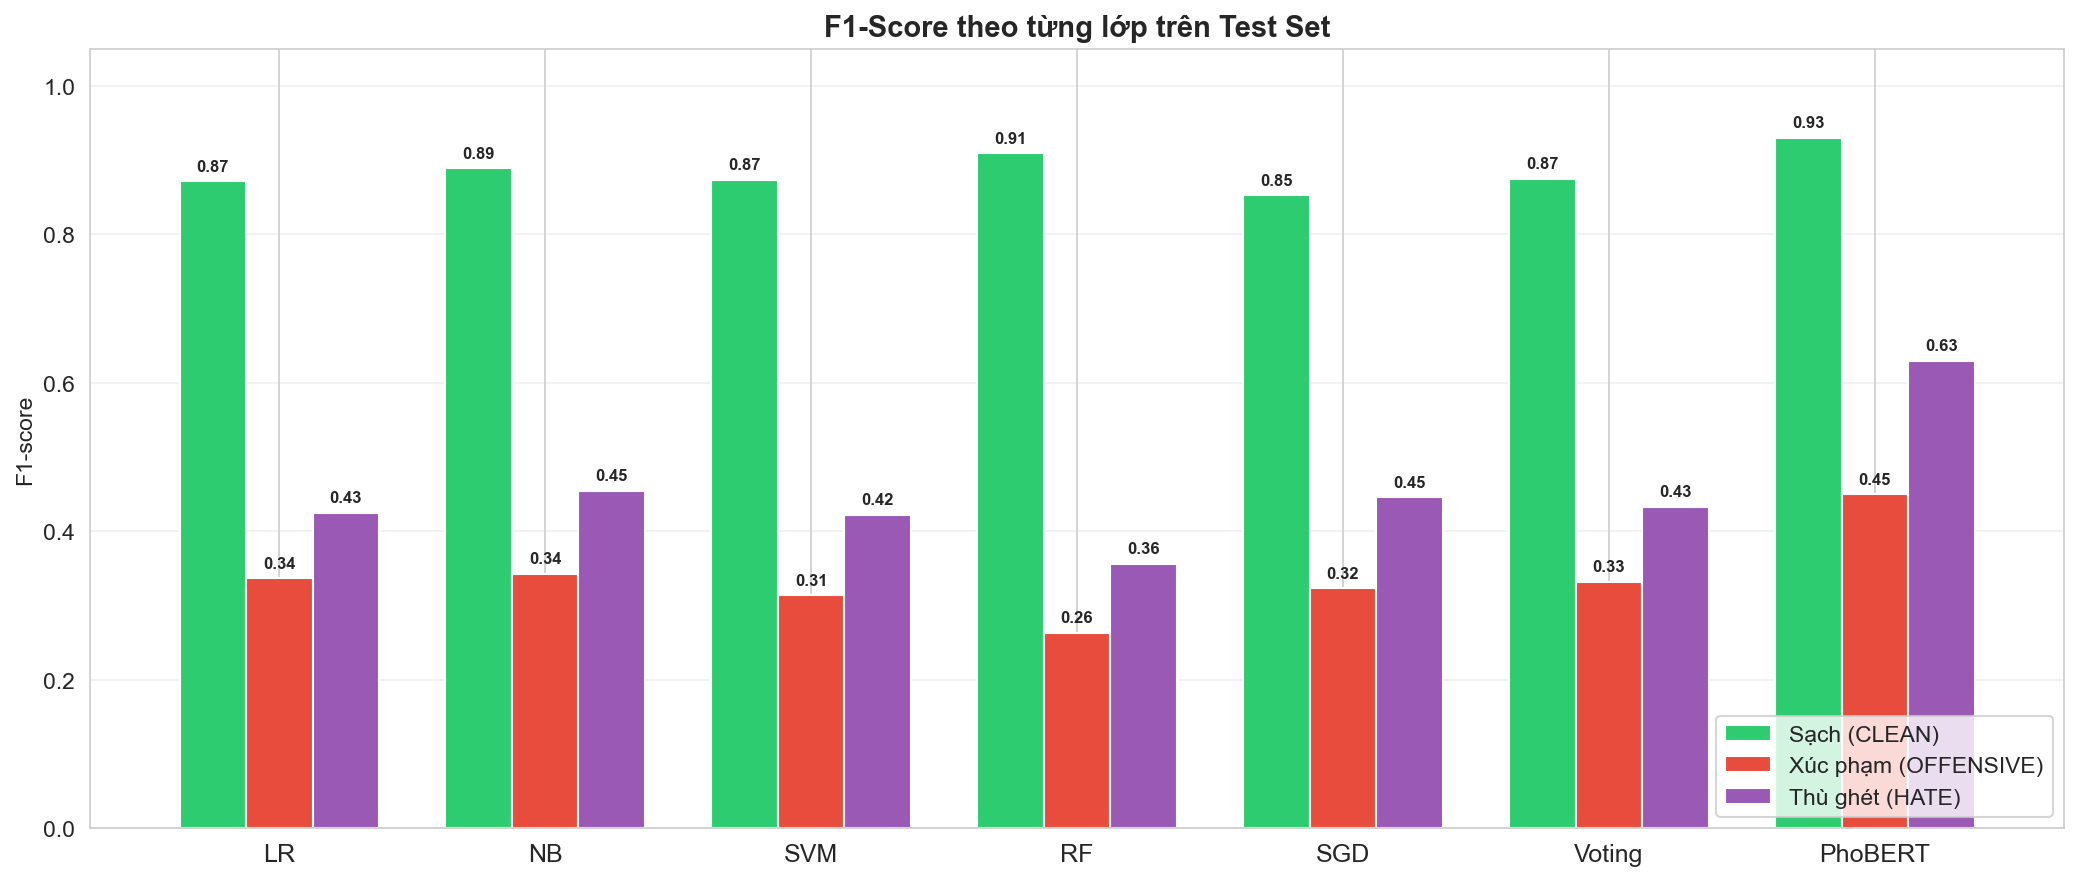
\includegraphics[width=0.8\textwidth]{figures/f1_per_class.png}
\caption{F1-Score theo từng lớp cho các mô hình truyền thống}
\label{fig:f1_per_class}
\end{figure}

Hình~\ref{fig:model_comparison} so sánh Accuracy và F1-weighted giữa các mô hình.

\begin{figure}[H]
\centering

\includegraphics[width=0.75\textwidth]{figures/model_comparison.png}
\caption{So sánh Accuracy và F1-weighted giữa các mô hình trên tập Test}
\label{fig:model_comparison}
\end{figure}

\textbf{Nhận xét tổng quan:}
\begin{itemize}
    \item \textbf{PhoBERT} đạt hiệu suất cao nhất (F1-weighted = 0.8637, F1-macro = 0.6703), vượt trội so với các mô hình truyền thống nhờ khả năng nắm bắt ngữ nghĩa sâu qua pre-trained language model.
    \item Trong nhóm mô hình truyền thống, \textbf{Random Forest} và \textbf{Multinomial NB} bất ngờ đạt F1-weighted cao nhất ($\approx$0.81), vượt qua cả Voting Ensemble.
    \item \textbf{Voting Ensemble} không đạt hiệu quả như kỳ vọng do các mô hình thành viên (LR, SVM, SGD) có cùng bias tương tự (đều là tuyến tính), làm giảm tính đa dạng cần thiết cho ensemble.
    \item Lớp OFFENSIVE (nhãn 1) luôn có F1-score thấp nhất ở mọi mô hình (0.30--0.45), phản ánh bản chất khó phân loại của bình luận xúc phạm nhẹ so với bình luận sạch.
\end{itemize}
